\documentclass[spanish,a4paper]{beamer}%
%,aspectratio=169

%% CUSTOM COLOR
\definecolor{azuremist}{rgb}{0.94, 1.0, 1.0}
\definecolor{ashgrey}{rgb}{0.7, 0.75, 0.71}
\definecolor{myyellow}{rgb}{.9,.9,.1}
\definecolor{cadmiumorange}{rgb}{0.93, 0.53, 0.18}
\definecolor{carminered}{rgb}{1.0, 0.0, 0.22}
\definecolor{carmine}{rgb}{0.59, 0.0, 0.09}
\definecolor{chromeyellow}{rgb}{1.0, 0.65, 0.0}

%% USE PACKAGE
\usepackage[spanish, es-tabla]{babel}
\usepackage{float}
\usepackage[utf8]{inputenc}
\usepackage{color}
\usepackage{amsmath}
\usepackage{amsfonts}
\usepackage{amssymb}
\usepackage{cite}
\usepackage{epstopdf}
\usepackage{array}
\usepackage{multirow}
\usepackage{multicol}
\usepackage{hyperref}
\usepackage{nameref}
\usepackage{graphicx}
\usepackage[font={tiny,color=ashgrey},skip=0pt]{caption}
\usepackage[font={tiny,color=ashgrey},skip=0pt]{subcaption}

%\usepackage[ backend=biber,style=authortitle,]{biblatex}

\usetheme{Berlin}%Berlin}Luebeck
\usecolortheme[named=chromeyellow]{structure}
%\usecolortheme{whale}

\sloppy
\epstopdfsetup{outdir=./pdf}

%%% NEW COMMANDS
\makeatletter
\let\beamer@writeslidentry@miniframeson=\beamer@writeslidentry%
\def\beamer@writeslidentry@miniframesoff{%
  \expandafter\beamer@ifempty\expandafter{\beamer@framestartpage}{}% does not happen normally
  {%else
    % removed \addtocontents commands
    \clearpage\beamer@notesactions%
  }
}
\newcommand*{\miniframeson}{\let\beamer@writeslidentry=\beamer@writeslidentry@miniframeson}
\newcommand*{\miniframesoff}{\let\beamer@writeslidentry=\beamer@writeslidentry@miniframesoff}

\setbeamertemplate{headline}
{%
  \begin{beamercolorbox}[colsep=1.5pt]{upper separation line head}
  \end{beamercolorbox}
  \begin{beamercolorbox}{section in head/foot}
    \vskip2pt\insertsectionnavigationhorizontal{\paperwidth}{}{}\vskip2pt
  \end{beamercolorbox}%
  \ifbeamer@theme@subsection%
    \begin{beamercolorbox}[colsep=1.5pt]{middle separation line head}
    \end{beamercolorbox}
    \begin{beamercolorbox}[ht=2.5ex,dp=1.125ex,%
      leftskip=.3cm,rightskip=.3cm plus1fil]{subsection in head/foot}
      \usebeamerfont{subsection in head/foot}\insertsubsectionhead
    \end{beamercolorbox}%
  \fi%
  \begin{beamercolorbox}[colsep=1.5pt]{lower separation line head}
  \end{beamercolorbox}
}
\makeatother
\setbeamerfont{block body}{size=\small}

\makeatletter
	\newcommand*{\currentname}{\@currentlabelname}
	\newcommand{\resCondPath}{\graphicspath{{./figuras/Resultados/conduccion/}}}
	\newcommand{\resRadPath}{\graphicspath{{./figuras/Resultados/radiacion/}}}
	\newcommand{\resDiffMatEspPath}{\graphicspath{{./figuras/Resultados/DiffMatEsp/} }}
	\newcommand{\resRelPath}{\graphicspath{{./figuras/Resultados/RelacionCondRad/}}}
	\newcommand{\generalPath}{\graphicspath{{./figuras/}}}
\makeatother

%\usepackage{etoc}
%para generar índice con hipervínculos



%parametros del documento (sus propiedades)
\hypersetup{
    pdftitle={Martin Augusto Reigadas Teran - TFG - 2022},
    pdfsubject={TFG - 2022},
    pdfauthor={Martin Augusto Reigadas Teran},
    pdfkeywords={termo-fotovoltaica} {campo cercano} {recuperación de calor},
    colorlinks,
    citecolor=ashgrey,
    filecolor=ashgrey,
    linkcolor=ashgrey,
    urlcolor=ashgrey,
}

%%%   TITLE PAGE
\title[\color{white} \tiny Modelado y simulación de espaciadores nanométricos para su aplicación en dispositivos TPVs de campo cercano]{\LARGE Modelado y simulación de espaciadores nanométricos para su aplicación en dispositivos TPVs de campo cercano}
\author[Martin Augusto Reigadas Teran]{\large Martin Augusto Reigadas Teran}
\institute{Universidad Politécnica de Madrid}
\date{Septiembre, 2022}

 %%% TABLES OF CONTENTS
\AtBeginSection[]
{
\hypersetup{linkcolor=black}
   \begin{frame}<beamer>{\currentname}
        \tableofcontents[currentsection,currentsubsection,hideothersubsections, 
    sectionstyle=show/shaded,subsectionstyle=hide]
   \end{frame}
	\hypersetup{linkcolor=ashgrey}
}
\AtBeginSubsection[]
{
\hypersetup{linkcolor=black}
   \begin{frame}<beamer>{\currentname}
        \tableofcontents[currentsubsection,hideothersubsections, 
    sectionstyle=hide,subsectionstyle=show/shaded/hide]
   \end{frame}
	\hypersetup{linkcolor=ashgrey}
}


\begin{document}
\generalPath
	%\metroset{block=fill}

	%% TITLE PAGE
	{
		\setbeamercolor{author in head/foot}{use=palette secondary, fg=palette secondary.bg} 
		\setbeamercolor{institute in head/foot}{use=palette secondary, fg=palette secondary.bg}
		\setbeamercolor{section in head/foot}{use=palette tertiary, fg=palette tertiary.bg}
		\setbeamercolor{subsection in head/foot}{use=palette secondary, fg=palette secondary.bg} 

		\begin{frame}
			\titlepage
			\begin{minipage}[l]{0.48\textwidth}
			\begin{flushleft}
				\footnotesize \itshape  Tutor: Pablo García-Linares Fontes\\
				\tiny Departamento de Ingeniería Eléctrica, Electrónica, Automática y
		Física Aplicada		
			\end{flushleft}
			\end{minipage}\hfill
			\begin{minipage}[r]{0.48\textwidth}
			\begin{flushright}
				\footnotesize \itshape Cotutora: Esther López Estrada\\
				 \tiny Instituto de Energía Solar\\
				
						
			\end{flushright}
			\end{minipage}
		\end{frame}
	}

	%%  TABLA DE CONTENIDOS
	{
		\setbeamercolor{section in head/foot}{use=palette tertiary, fg=palette tertiary.bg}
		\begin{frame}{Tabla de Contenidos}
				\hypersetup{linkcolor=black}
				\tableofcontents[hideallsubsections]
		\end{frame}
	}

	%% INTRODUCCION
	\section{Introducción}
	\begin{frame}{Introducción}

\only<1>{
	\vspace{10pt}	
	%% FIGURAS DE DEMANDAS
	\begin{figure}
		\centering
		\begin{subfigure}[b]{0.58\textwidth}
		\centering
			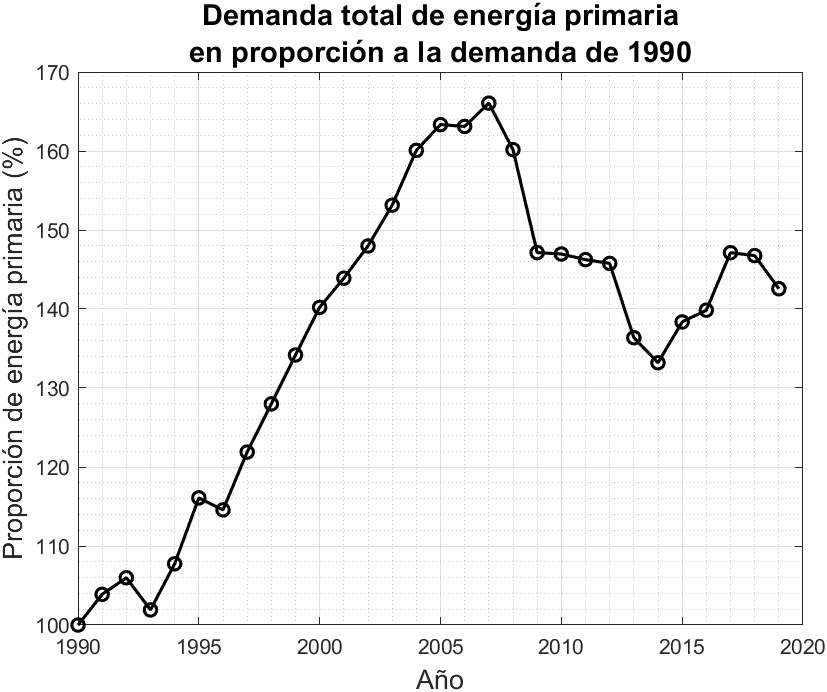
\includegraphics[width=\textwidth]{DemandaEnergiaPrimariaProporcion1990.png}
			\caption*{Fuente de datos: Ministerio para la transición ecológica y el reto demográfico de España.}
		\end{subfigure} \hfill
		\begin{subfigure}[b]{0.4\textwidth}
			\centering
			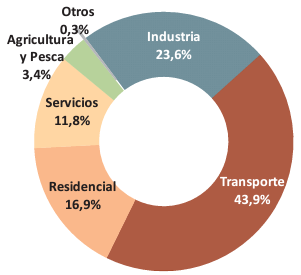
\includegraphics[width=\textwidth]{consumoEnergiaFinalPorSectores_2019.png}
			\caption*{Fuente: Ministerio para la transición ecológica y el reto demográfico de España (2019).}
		\end{subfigure}
		\label{fig:demandaYconsumo}
	\end{figure}
}
\only<2->{
\vspace{-10pt}
%%  FIGURAS SISTEMAS MECANICOS DE GENERACION
\begin{figure}[htbp]
	\centering
	\onslide<2->{
	\begin{subfigure}[b]{0.55\textwidth}
		\centering
			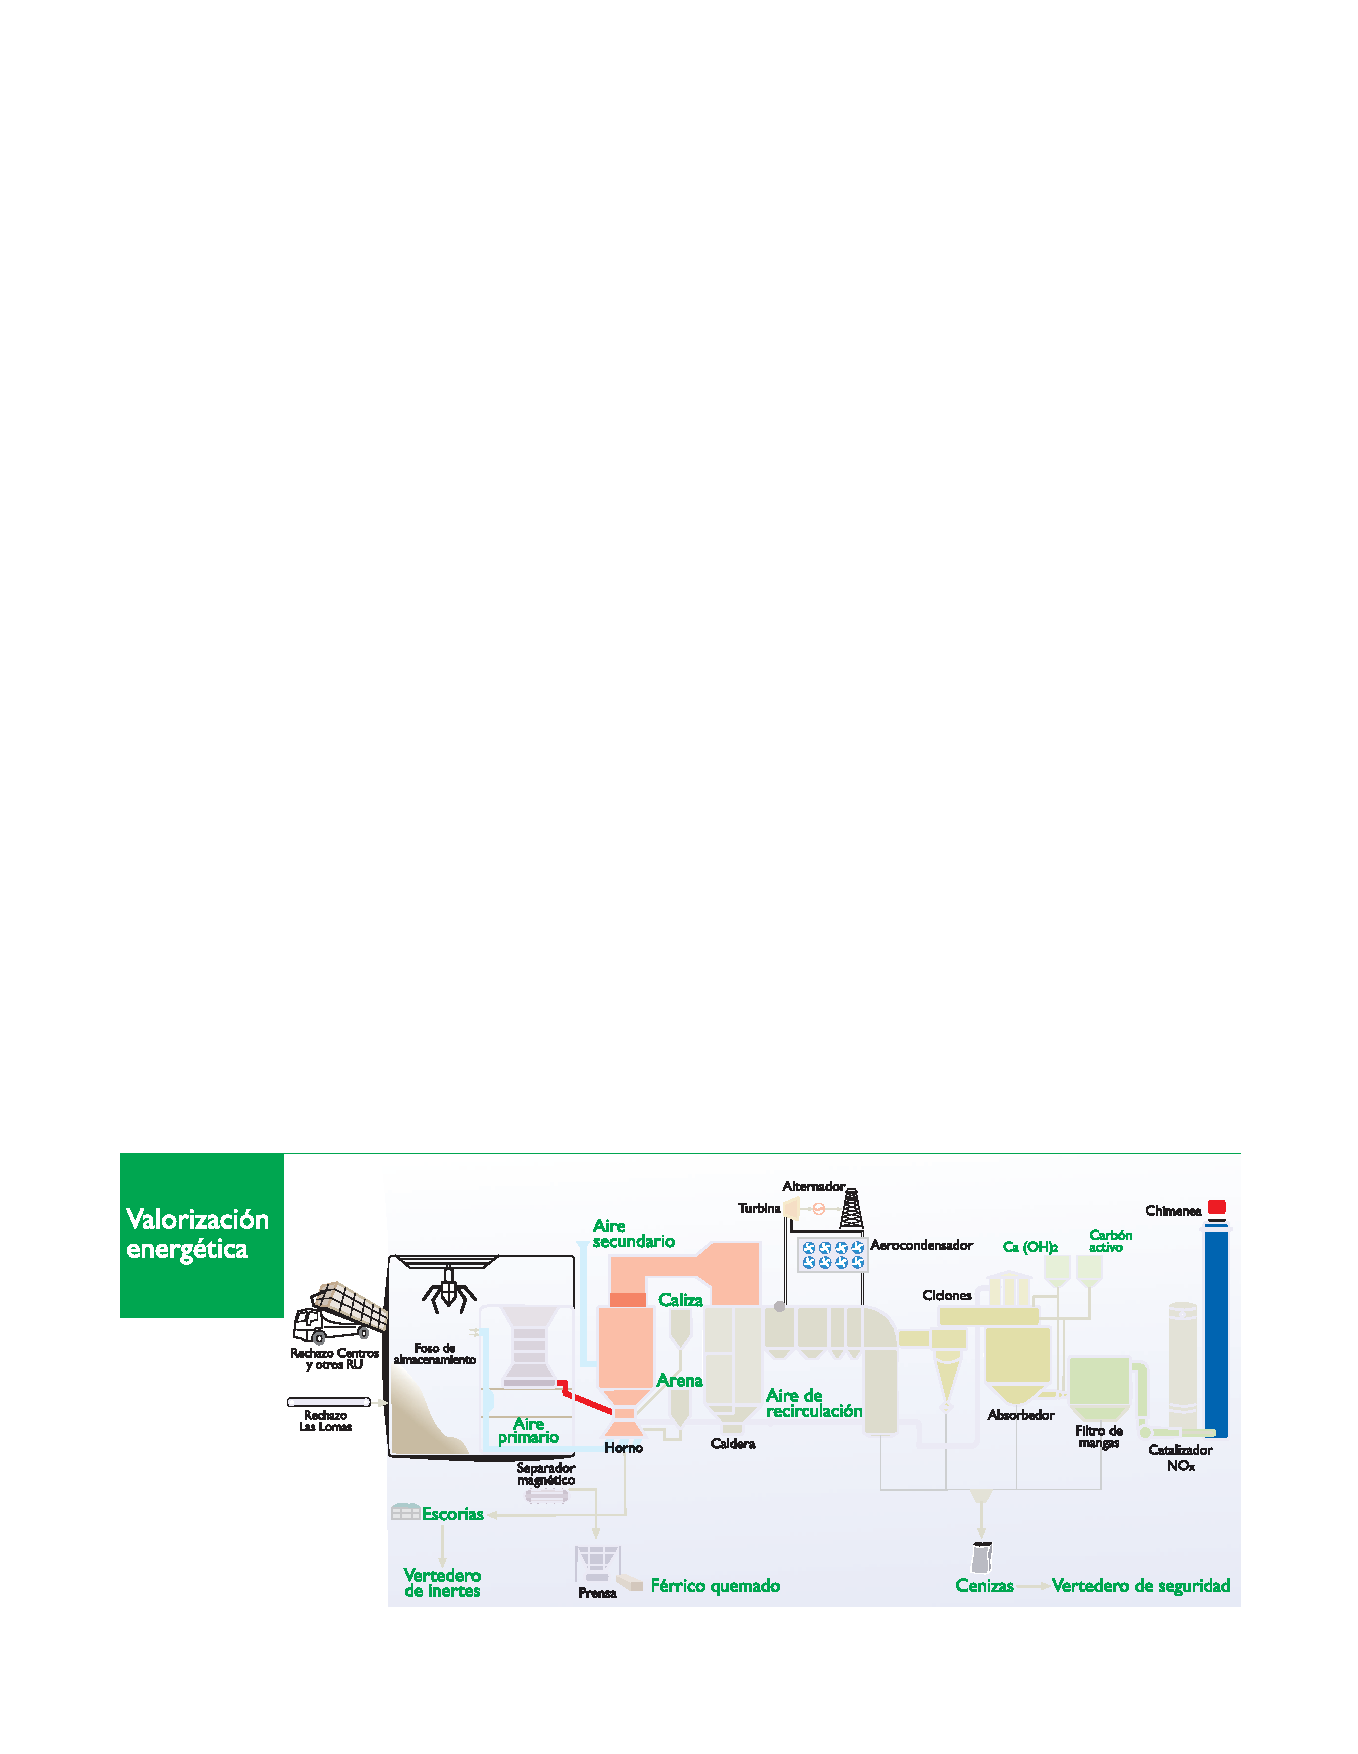
\includegraphics[width=\textwidth]{esquemasLomasValorizacion}
			\caption*{Fuente: Ayuntamiento de Madrid.}
	\end{subfigure}\hfill}
	%
	\onslide<3->{
	\begin{subfigure}[b]{0.4\textwidth}
		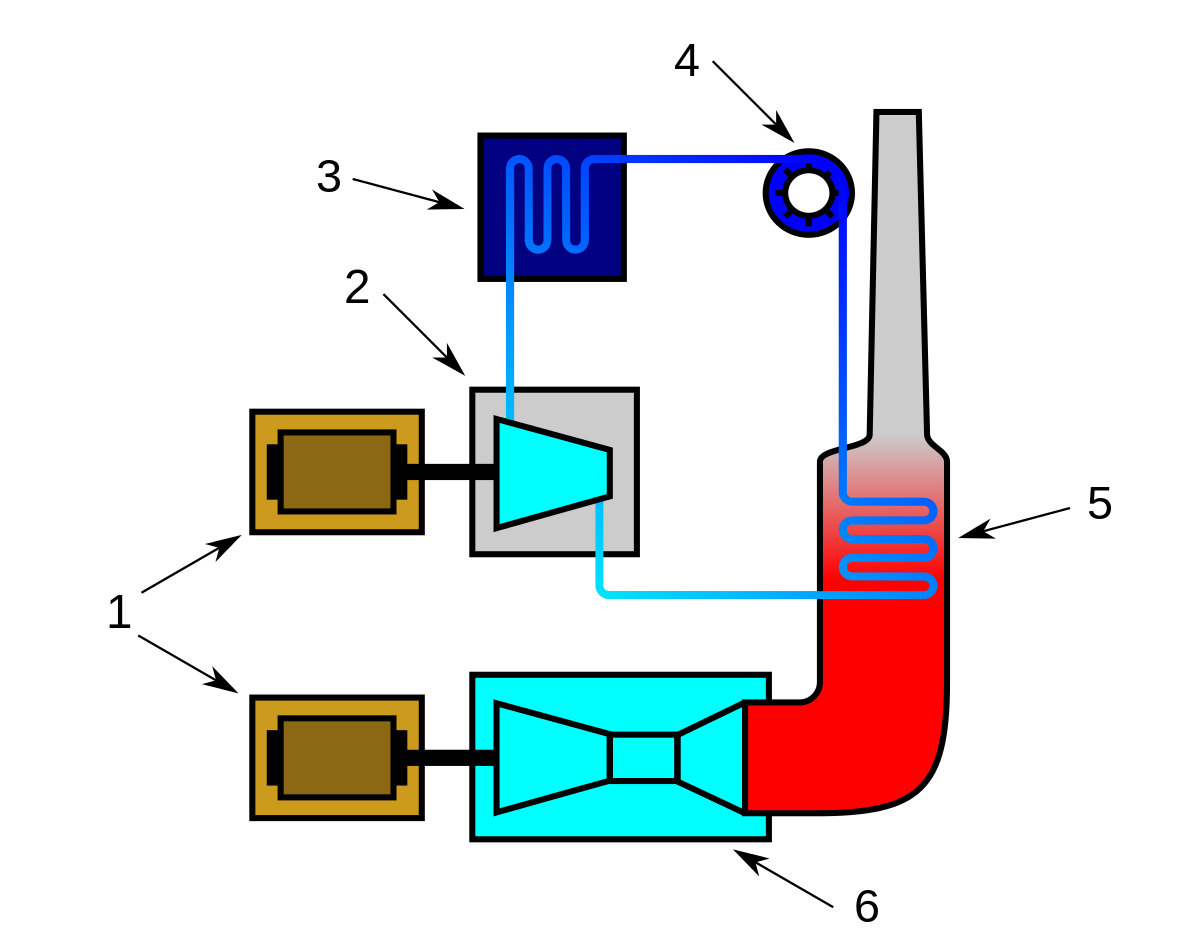
\includegraphics[width=\textwidth]{cicloCombinado}
		\caption*{Ciclo combinado. Fuente: Wikipedia.}
	\end{subfigure} \hfill}
	%
	\onslide<4->{
	\begin{subfigure}[b]{0.38\textwidth}
	\vspace{-5pt}
		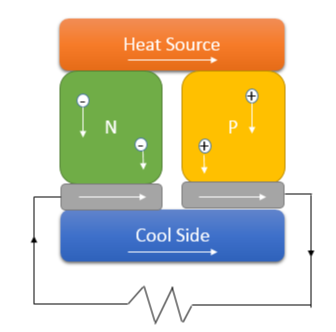
\includegraphics[height=0.4\textheight,width=\textwidth,angle=0]{TEG}
		\caption*{TEG. Fuente: \cite{TEG5efficiency}}
	\end{subfigure}
	\hfill}
	\onslide<5->{
	\begin{subfigure}[b]{0.48\textwidth}
	\vspace{-1cm}
		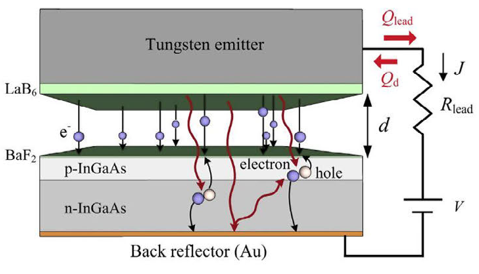
\includegraphics[width=\textwidth]{iTPV}
		\caption*{iTPV. Fuente: \cite{Thermoionic_nTPV_DATAS201910}}
	\end{subfigure} }
%
\label{fig:valdemingomez_cc_TEG_iTPV}
\end{figure}
}
	\end{frame}

%%  ESTADO DEL ARTE 
	\section{Estado del arte}
	\subsection{Termo-fotovoltaica}
	\begin{frame}{Termo-fotovoltaica}
		\begin{figure}[ht]
			\centering
			\only<1>{
			\begin{subfigure}[b]{0.48\textwidth}
				\centering
					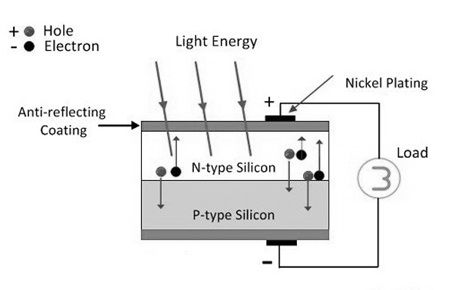
\includegraphics[width=1.00\textwidth]{PV_Effect}
				\caption*{Efecto fotovoltaico. Fuente: \cite{picPvEffect}}
				\label{fig:PV_Effect}
			\end{subfigure}
			}
			%
			\only<1->{
			\hfill
			\begin{subfigure}[b]{0.4\textwidth}
				\centering
					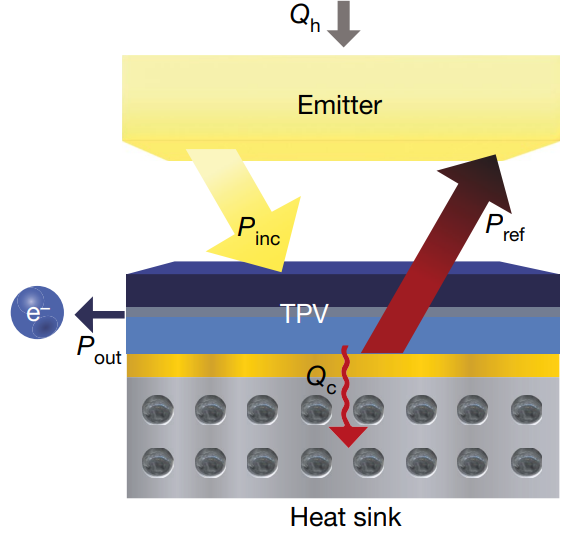
\includegraphics[width=1.00\textwidth]{TPV_40_BSR}
				\caption*{Efecto fotovoltaico. Fuente: \cite{thermophotovoltaic_40}}
				\label{fig:PV_Effect}
			\end{subfigure}
			}
			%
			\only<2->{
			\hfill
			\begin{subfigure}[b]{0.48\textwidth}
					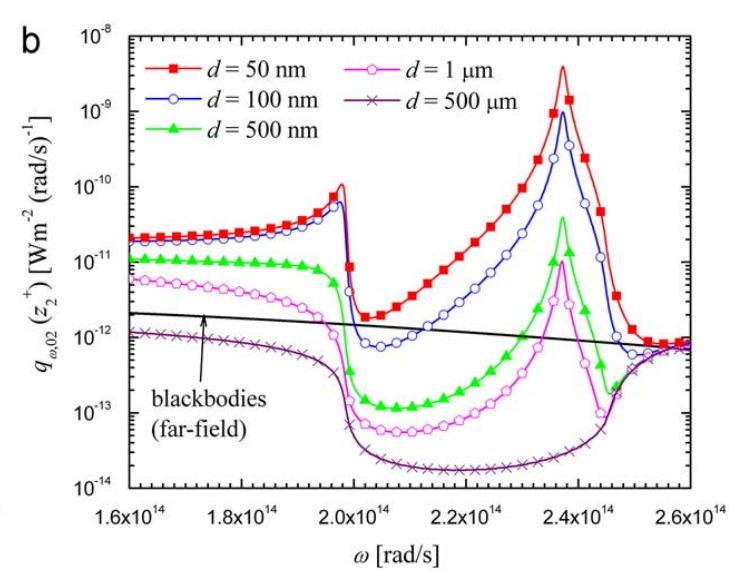
\includegraphics[width=1.00\textwidth]{graficaDiff_dc_fullEqu}
				\caption*{Radiación campo cercano. Fuente: \cite{nfTPV_fullEquations}}
				\label{fig:PV_Effect}
			\end{subfigure}
			}
		\label{fig:TPV}
		\end{figure}
		
	\end{frame}
	\subsection{Campo cercano}
	\begin{frame}{Campo cercano}
		
	\end{frame}
%%  MATERIALES Y HERRAMIENTAS
	\section{Materiales y herramientas}
	\begin{frame}{Materiales y herramientas}
		
	\end{frame}


%% METODOS
	\section{Métodos}
	\begin{frame}{Métodos}
		
	\end{frame}

%% RESULTADOS Y DISCUSIÓN
\graphicspath{{./figuras/Resultados}}

	\section{Resultados y discusión}
	\begin{frame}{Resultados y discusión}
	%\localtableofcontents
	\hypersetup{linkcolor=black}
	%\onehalfspacing
		\tableofcontents[currentsubsection,hideothersubsections, 
    sectionstyle=hide,subsectionstyle=show/show/hide]
		%\hypersetup{linkcolor=ashgrey}
	\end{frame}
	
	\subsection{nTPV Si-SiO2-Si}
	\begin{frame}{nTPV Si-SiO2-Si}
		\only<1-2>{ %%%   CONDUCCION
			\frametitle{Conducción}
			\resCondPath
			\begin{columns}
			\column{.5\textwidth}
					\vspace{-10pt}
					\begin{block}{\centering Sin Rc}
					\end{block}
					\vspace{-10pt}
					\begin{figure}%
							\centering
							\begin{subfigure}[b]{0.9\columnwidth}
									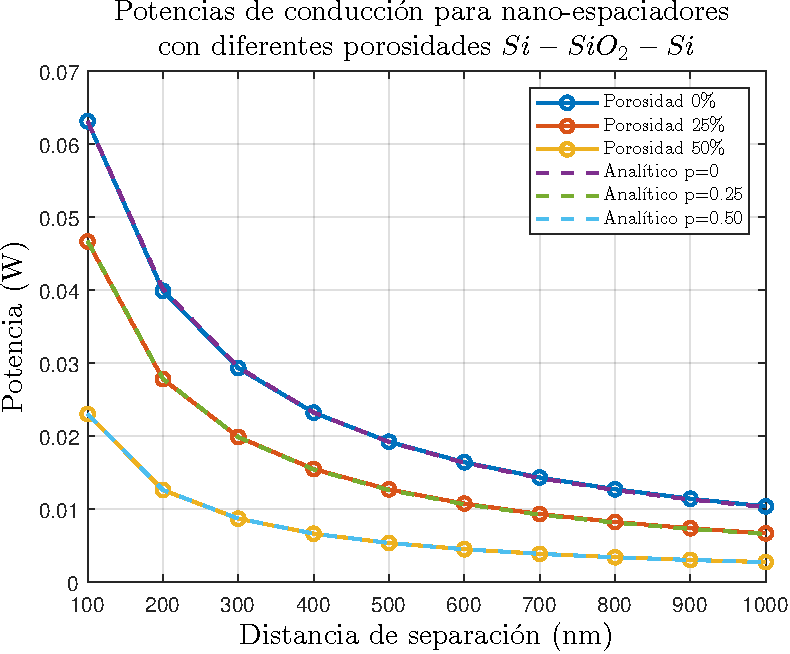
\includegraphics[width=\textwidth]{Ppor_SiSiO2Si}
							\end{subfigure}\hfill \vfill
							\begin{subfigure}[b]{0.8\columnwidth}
									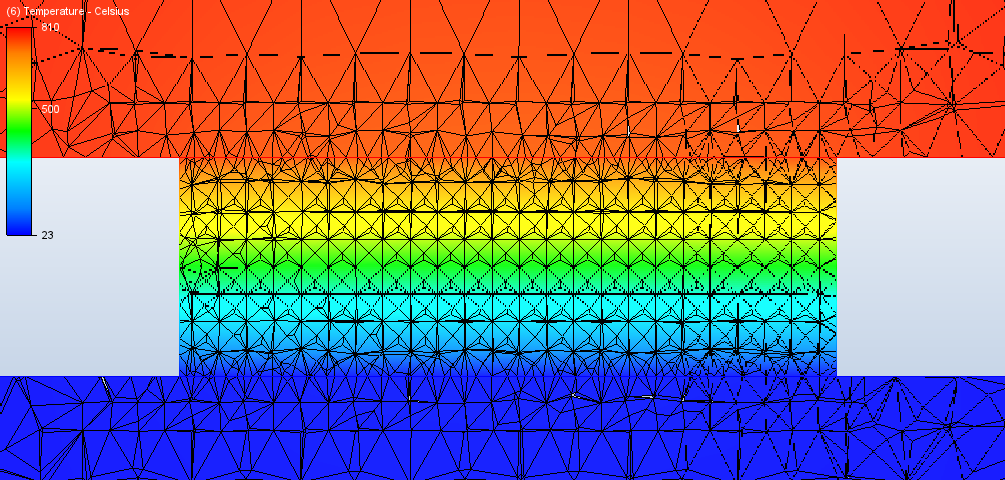
\includegraphics[width=\textwidth]{SiSiO2Si_1000nm_Plane}%
							\end{subfigure}
							\label{fig:SiSiO2Si_cond}%Pn_SiCSiO2Ge
					\end{figure}
			\column{.5\textwidth}
			\vspace{-10pt}
					\begin{block}{\centering Con Rc}
					\end{block}
			\vspace{-10pt}
			\begin{figure}%
			\centering
			\begin{subfigure}[b]{0.9\columnwidth}
				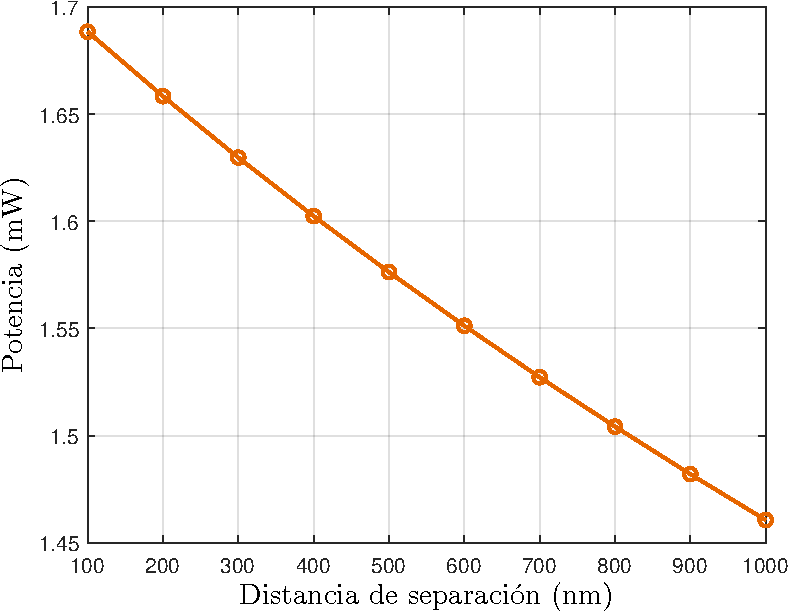
\includegraphics[width=\textwidth]{Prc2_SiSiO2Si}%
			\end{subfigure}
				\hfill \vfill
			\begin{subfigure}[b]{0.8\columnwidth}
				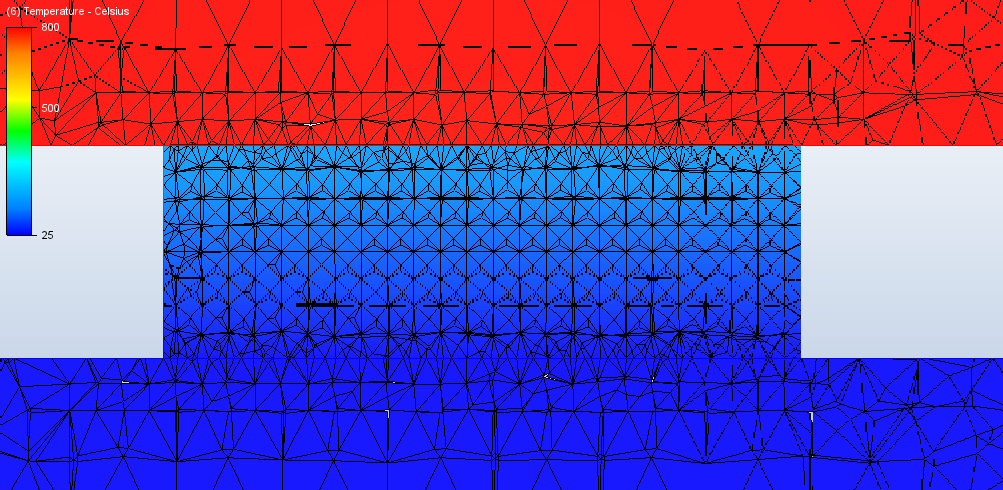
\includegraphics[width=\textwidth]{SiSiO2Si_1000nm_Plane_Rc}
			\end{subfigure}
				\label{fig:SiSiO2Si_condRc}%
			\end{figure}
			\end{columns}			
		}
		%%%  RADIACION
		\only<3>{
			\frametitle{Radiación}
			\resRadPath
			\begin{columns}
			%%
				\column{.5\textwidth}
					%\vspace{-10pt}
						\begin{block}{\centering Por longitud de onda}
						\end{block}
					\vspace{15pt}
						\begin{figure}[h]%
								\centering
										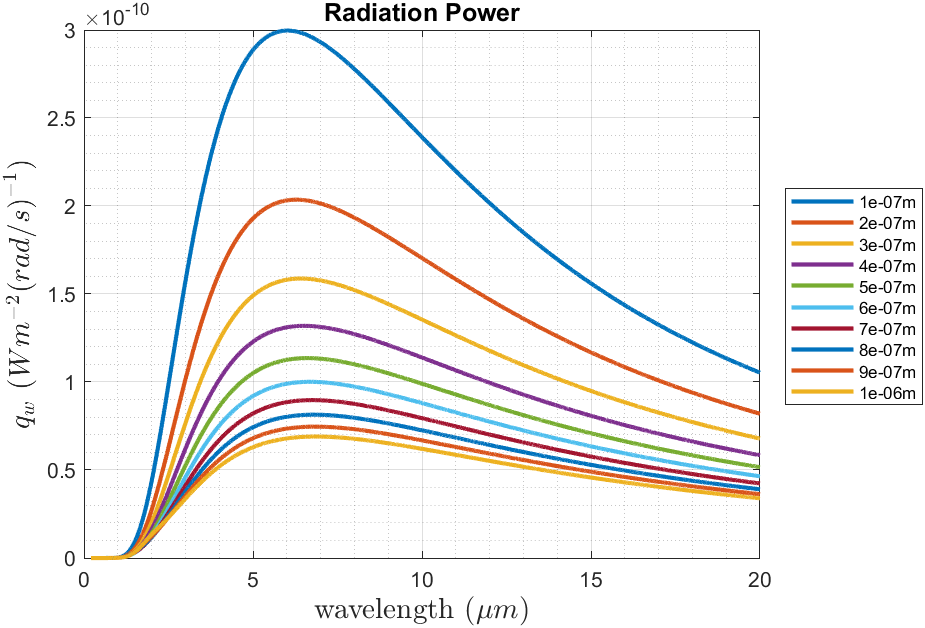
\includegraphics[width=\columnwidth]{SiSi_ds}
								\label{fig:SiSiO2Si_rad}%Pn_SiCSiO2Ge
						\end{figure}
						\vfill
						%%
				\column{.5\textwidth}
					\vspace{-10pt}
						\begin{block}{\centering En el rango de $E>1.1eV$}
							\end{block}
					\vspace{10pt}
						\begin{figure}[h]%
								\centering
										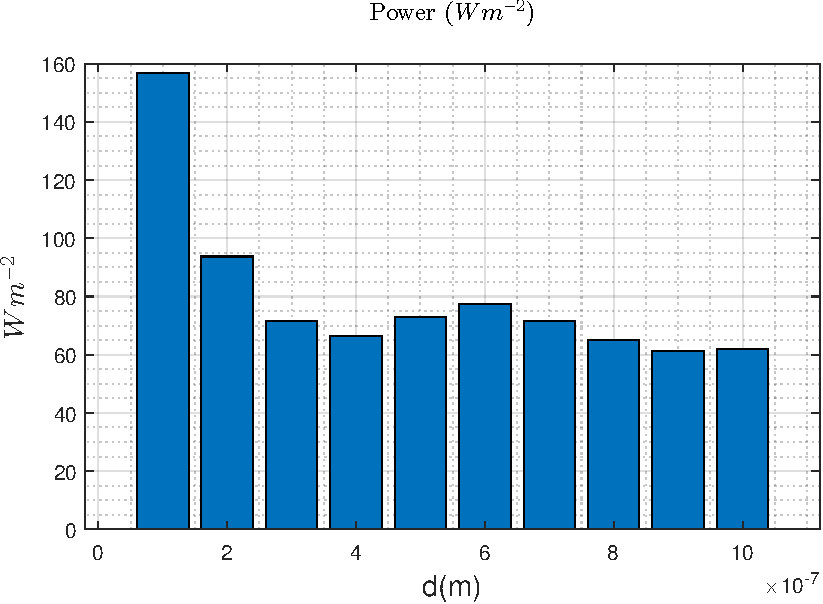
\includegraphics[width=\columnwidth]{p_11_SiSi}%
								\label{fig:SiSiO2Si_radInt}%
						\end{figure}
						\vfill
				\end{columns}		
		}
		%%%  DENSIDADES DE NANO-ESPACIADORES
		\only<4>{
			\frametitle{Densidades para $E>1.1eV$}
			\resRelPath
			\begin{columns}
			%%
				\column{.5\textwidth}
					%\vspace{-1cm}
						\begin{block}{\centering Sin Rc}
						\end{block}
					\vspace{10pt}
						\begin{figure}[h]%
								\centering
										\includegraphics[width=\columnwidth]{rel_SiSi11}
								\label{fig:SiSiO2Si_rel}%Pn_SiCSiO2Ge
						\end{figure}
						\vfill
						%%
				\column{.5\textwidth}
					\vspace{-12pt}
						\begin{block}{\centering Con Rc}
							\end{block}
					\vspace{10pt}
						\begin{figure}[h]%
								\centering
										\includegraphics[width=\columnwidth]{rel_SiSi11_Rc}%
								\label{fig:SiSiO2Si_relRc}%
						\end{figure}
						\vfill
				\end{columns}		
		}
	\end{frame}
	
	\subsection{nTPV Si-SiO2-Ge}
	\begin{frame}{nTPV Si-SiO2-Ge}
			\only<1>{ %%%   CONDUCCION
			\frametitle{Conducción}
			\resCondPath
			\begin{columns}
			%%
				\column{.5\textwidth}
					%\vspace{-10pt}
						\begin{block}{\centering Sin Rc}
						\end{block}
					\vspace{15pt}
						\begin{figure}[h]%
								\centering
										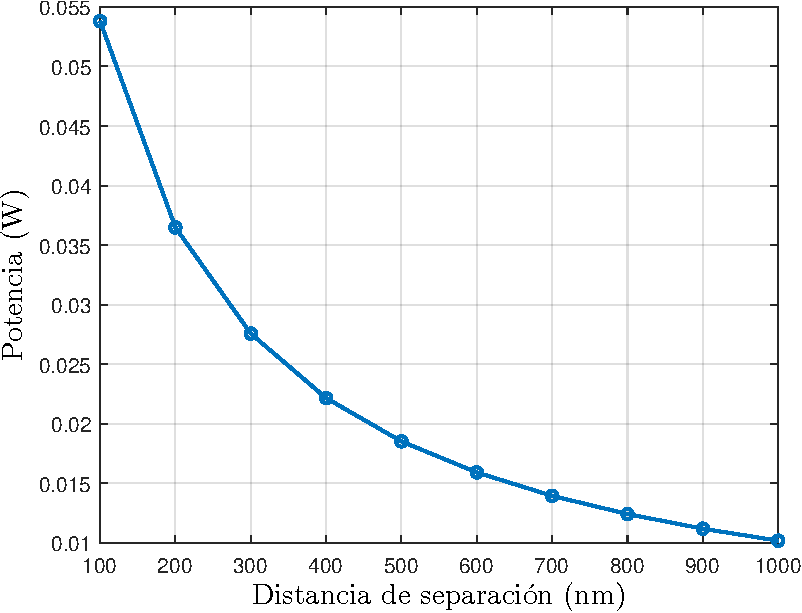
\includegraphics[width=\columnwidth]{Pn_SiSiO2Ge}
								\label{fig:SiSiO2Ge_cond}%Pn_SiCSiO2Ge
						\end{figure}
						\vfill
						%%
				\column{.5\textwidth}
					\vspace{-10pt}
						\begin{block}{\centering En el rango de $E>0.7eV$}
							\end{block}
					\vspace{10pt}
						\begin{figure}[h]%
								\centering
										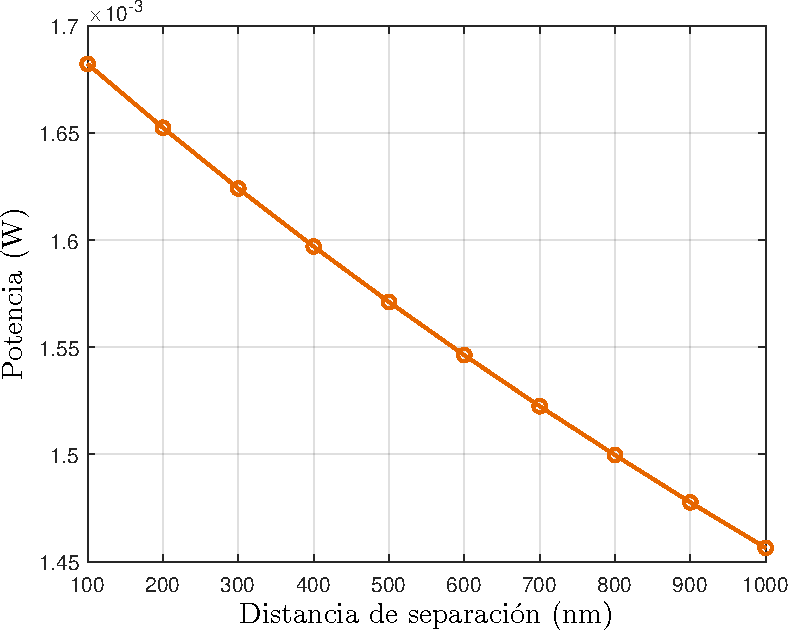
\includegraphics[width=\columnwidth]{Prc2_SiSiO2Ge}%
								\label{fig:SiSiO2Ge_condRc}%
						\end{figure}
						\vfill
				\end{columns}							
		}
		%%%  RADIACION
		\only<2>{
			\frametitle{Radiación}
			\resRadPath
			\begin{columns}
			%%
				\column{.5\textwidth}
					%\vspace{-10pt}
						\begin{block}{\centering Por longitud de onda}
						\end{block}
					\vspace{15pt}
						\begin{figure}[h]%
								\centering
										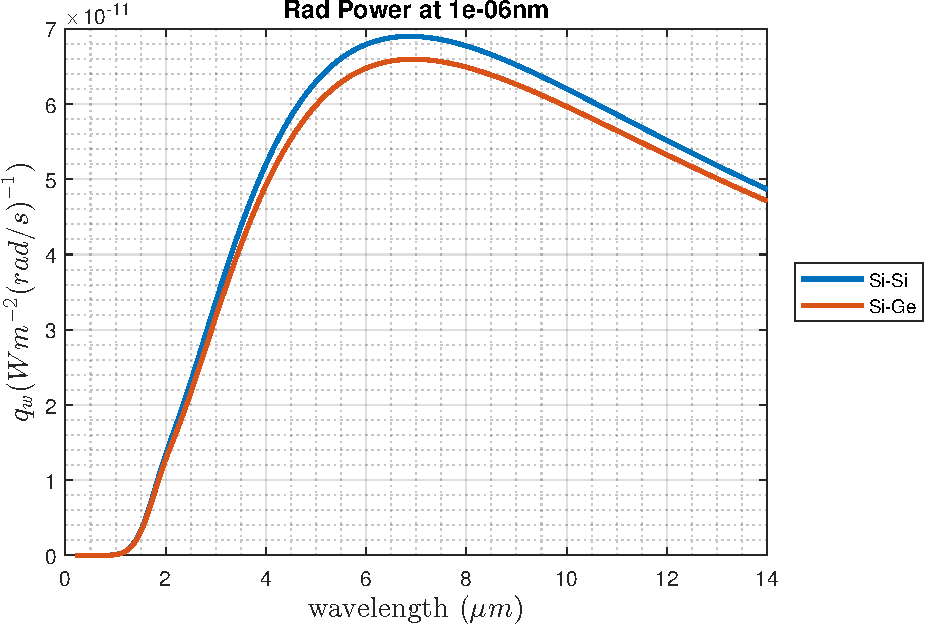
\includegraphics[width=\columnwidth]{SiSi_vs_SiGe}
								\label{fig:SiSivsSiGe_rad}%Pn_SiCSiO2Ge
						\end{figure}
						\vfill
						%%
				\column{.5\textwidth}
					\vspace{-10pt}
						\begin{block}{\centering En el rango de $E>0.7eV$}
							\end{block}
					\vspace{10pt}
						\begin{figure}[h]%
								\centering
										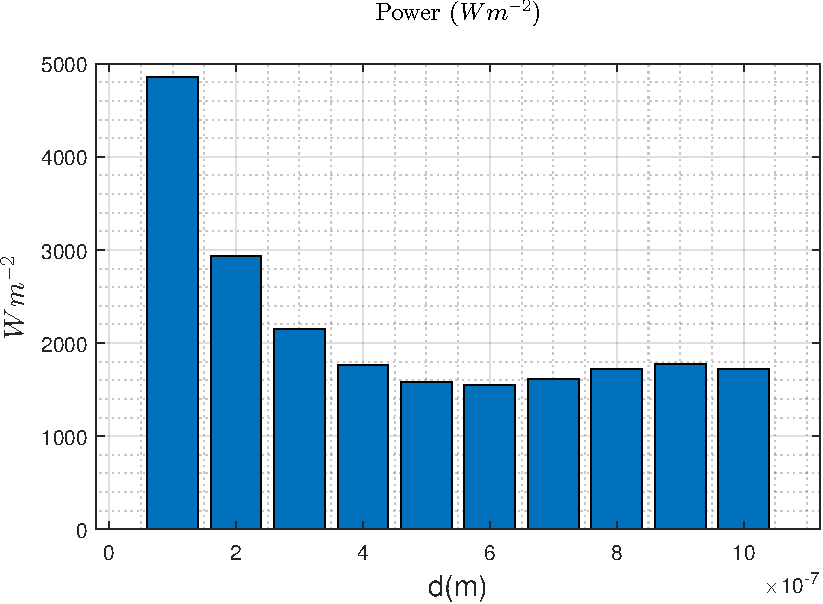
\includegraphics[width=\columnwidth]{p_Eg_SiGe}%
								\label{fig:SiSiO2Ge_radInt}%
						\end{figure}
						\vfill
				\end{columns}		
		}
		%%%  DENSIDADES DE NANO-ESPACIADORES
		\only<3>{
			\frametitle{Densidades para $E>0.7eV$}
			\resRelPath
			\begin{columns}
			%%
				\column{.5\textwidth}
					%\vspace{-1cm}
						\begin{block}{\centering Sin Rc}
						\end{block}
					\vspace{10pt}
						\begin{figure}[h]%
								\centering
										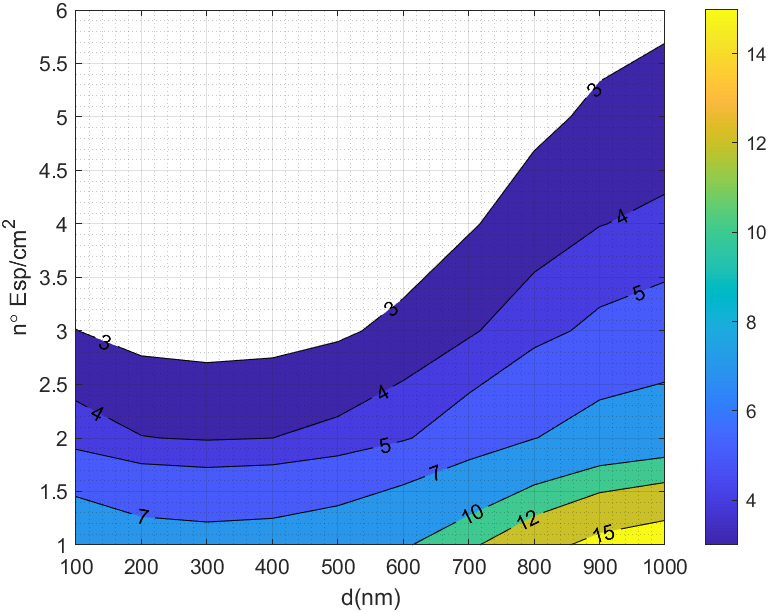
\includegraphics[width=\columnwidth]{SiGe}
								\label{fig:SiSiO2Ge_rel}%Pn_SiCSiO2Ge
						\end{figure}
						\vfill
						%%
				\column{.5\textwidth}
					\vspace{-12pt}
						\begin{block}{\centering Con Rc}
							\end{block}
					\vspace{10pt}
						\begin{figure}[h]%
								\centering
										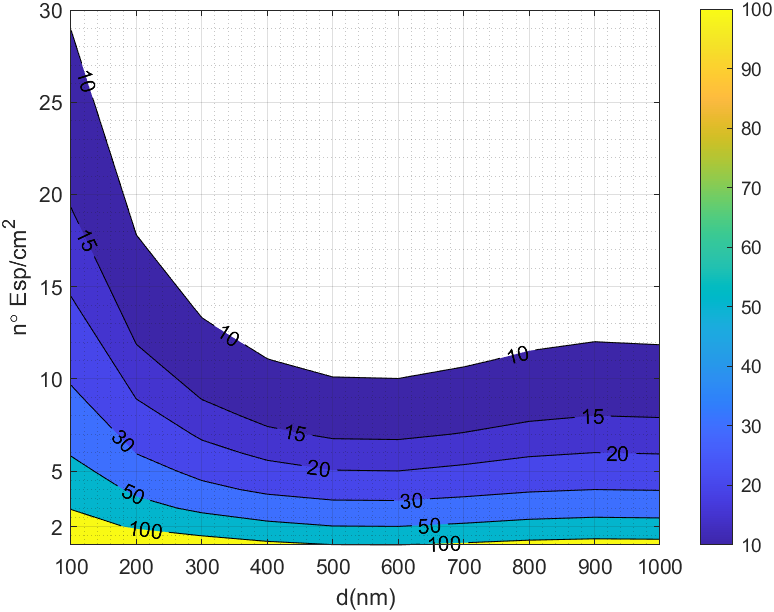
\includegraphics[width=\columnwidth]{SiGe_Rc}%
								\label{fig:SiSiO2Ge_relRc}%
						\end{figure}
						\vfill
				\end{columns}		
		}
	\end{frame}
	
	\subsection{nTPV SS-SiO2-Ge}
	\begin{frame}{nTPV SS-SiO2-Ge}
	
	\end{frame}
	
	\subsection{nTPV SiC-SiO2-Ge}
	\begin{frame}{nTPV SiC-SiO2-Ge}
	
	\end{frame}
	
	\subsection{Densidad de carga}
	\begin{frame}{Densidad de carga}
	
	\end{frame}
	
	\subsection{Nano-espaciadore de Si}
	\begin{frame}{Nano-espaciadore de Si}
	
	\end{frame}
%% CONCLUSIONES
	\section{Conclusiones}
	\begin{frame}{Conclusiones}
	\end{frame}
	\subsection*{Desarrollos a futuro}
	\begin{frame}{Desarrollos a futuro}
		
	\end{frame}
%% FINAL
	\miniframesoff
	\section{}
	\begin{frame}{References}
        \bibliographystyle{apalike}
				\tiny
        \bibliography{bibliografia/bibliografia}
				
\end{frame}

\end{document}
